\chapter{METODOLOGIA} 
\label{chap:metodologia}

A metodologia deste trabalho visa propor e investigar arquiteturas de \gls{AP} que unificam características radiômicas e características profundas. O modelo base selecionado é uma versão adaptada do trabalho de \cite{aiSelfAttentionBasedFusion2023}, mencionado nos trabalhos relacionados e o esquemático de sua arquitetura pode ser visto na Figura \ref{fig:fig008}. Importante ressaltar que o trabalho em questão é aplicado no cenário de câncer de pulmão de células não pequenas em imagens de \gls{TC} e este trabalho pretende aplicar o mesmo estudo no cenário de cardiomiopatia.

 Os experimentos foram divididos em duas fases. Na primeira fase, foi aplicado o modelo base, ao conjunto de dados público selecionado. Na etapa de pré-processamento desta fase, foram aplicadas diversas técnicas de aprendizado de máquina para extrair características manuais de imagens de \gls{RMC} e sua respectiva máscara, abrangendo textura, forma, escala de cinza, etc. Estas características serão chamadas, deste ponto em diante, de características radiômicas. Seguindo com o pré-processamento, as imagens de \gls{RMC} foram processadas por uma rede \textit{ResNet50} pré-treinada, extraindo características que serão intituladas de características profundas. As características profundas encapsulam informações semânticas de alto nível e de representação das imagens de \gls{RMC}. Estas características, radiômicas e profundas, são então fundidas em um vetor de características unificado e aplicado a um único bloco de autoatenção, e obtendo ao fim da arquitetura do modelo base, as classificação indicando se há ou não cardiomiopatia, ou seja, uma classificação binária.

Na segunda fase, diversas adaptações foram aplicadas ao modelo base com o intuito de aprimorar a robustez e a acurácia. Algumas das adaptações feitas consistem no aumento do tamanho dos vetores semânticos, também conhecidos na literatura como \textit{embeddings}, seu tamanho foi variado também entre $12$, $24$, $48$ e $64$, valores testados de forma análoga a um hiperparâmetro, com a premissa de preservar mais das informações originais ao custo do aumento quase irrelevante de custo computacional.

A concatenação dos \textit{embeddings} também foi adaptada se comparada ao modelo original. Na versão original a concatenação se dá na última dimensão enquanto que nas versões adaptadas se dá na primeira dimensão. Em termos práticos, na versão original dois vetores $1\text{x}12$ concatenados resultam em $1\text{x}24$, na abordagem adaptada resultam em $2\text{x}12$. 

A mudança na forma de concatenar é feita de forma proposital pois a versão adaptada conta com uma camada convolucional inédita se comparada com a versão original, visando extrair informação relevante da junção dos \textit{embeddings}. A versão adaptada adiciona também uma camada de atenção seletiva no formato de um bloco \gls{SE} que precede o bloco de autoatenção. Outra mudança na versão adaptada é o bloco de autoatenção ser aplicado $N$ vezes ao invés de uma única vez como acontece no modelo base trazendo uma perceptível melhora nos resultados. Lembrando que ambos mecanismos de atenção tem propostas diferentes, enquanto o bloco de atenção seletiva atua na relação entre os canais dos \textit{embeddings}, o bloco de autoatenção otimiza e pondera o vetor de características fundidas de forma eficaz. A intuição de aplicar mecanismos de atenção com propósitos diferentes vem do trabalho de \cite{yangNeuralNetworkDesign2024a}. 

A Figuras \ref{fig:fig015-01} e \ref{fig:fig015-02} demonstram o fluxograma do projeto na fase de pré-processamento e o fluxograma da execução da arquitetura proposta respectivamente.

\begin{figure}[H]
    \centering
    \caption{Fluxograma - Pré-Processamento}
    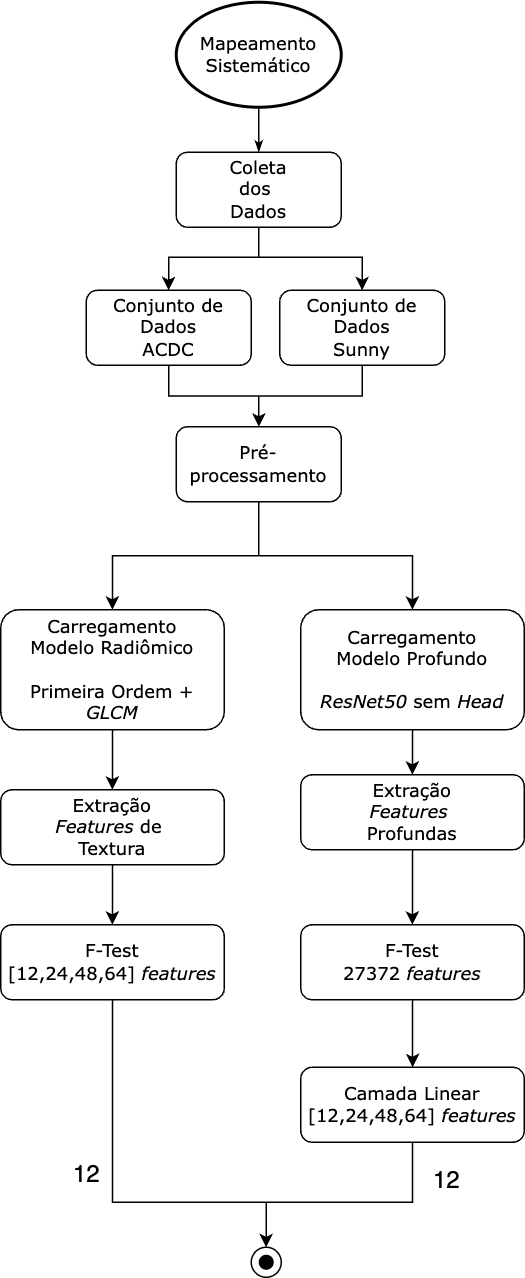
\includegraphics[scale=0.36]{figures/fig015-01.png}
    \caption*{Fonte: Autor}
    \label{fig:fig015-01}
\end{figure}

\begin{figure}[H]
    \centering
    \caption{Fluxograma - Arquitetura}
    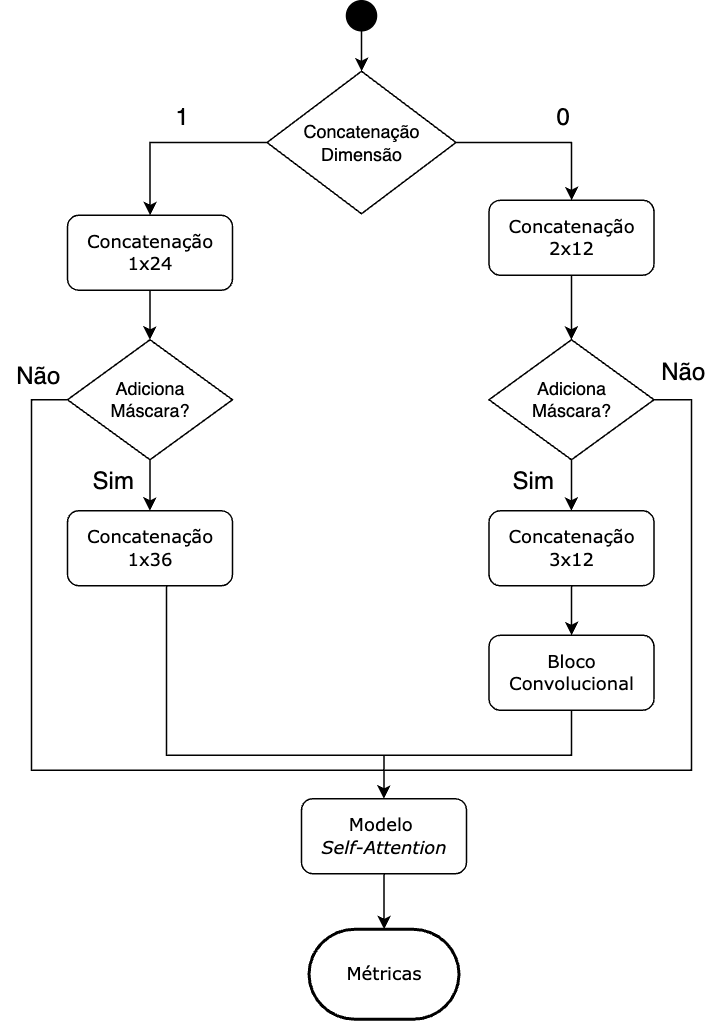
\includegraphics[scale=0.38]{figures/fig015-02.png}
    \caption*{Fonte: Autor}
    \label{fig:fig015-02}
\end{figure}

%--------------------------------------------------------
\section{BASES DE DADOS} 
\label{subsec:cap4_dataset}

Duas bases de dados foram utilizadas no experimento: o primeiro conjunto de dados é o \gls{ACDC}\footnote{https://www.creatis.insa-lyon.fr/Challenge/acdc/databases.html}. O segundo conjunto de dados é o SunnyBrook Cardiac Data (SCD) \footnote{https://www.cardiacatlas.org/sunnybrook-cardiac-data} \cite{radauEvaluationFrameworkAlgorithms2009}. Ambos conjuntos de dados são públicos e destinados a pesquisa.

\textcolor{red}{
O conjunto de dados ACDC é composto por $150$ imagens sendo $100$ para treino e $50$ para testes distribuídas em 5 classes igualmente distribuídas: \gls{DCM}, \gls{HCM}, \gls{NOR}, \gls{MINF} e \gls{RV}. O conjunto de dados SunnyBrook é composto por $45$ imagens sendo e, respeitando as proporções determinadas no ACDC, foi escolhido $30$ imagens para treino e $15$ para testes. As classes são NOR, IC, IC-I e HIP. Detalhes das classes são descritas nas seções que seguem destinadas a cada conjunto de dados.
}

%--------------------------------------------------------
\subsection{Conjunto de Dados ACDC} 
\label{subsec:cap4_acdc}

O conjunto de dados \gls{ACDC} foi criado a partir de exames clínicos reais adquiridos no hospital universitário de Dijon (França). Os dados adquiridos foram totalmente anonimizados e tratados de acordo com as regulamentações estabelecidas pelo comitê ético local do hospital de Dijon. O conjunto de dados cobre várias patologias bem definidas com casos suficientes para (1) treinar adequadamente métodos de aprendizado de máquina e (2) avaliar claramente as variações dos principais parâmetros fisiológicos obtidos a partir de cine-RM (em particular volume diastólico e fração de ejeção). O conjunto de dados é composto por $150$ exames (todos de pacientes diferentes) divididos em cinco subgrupos distribuídos de forma igualitária, sendo quatro patológicos e um grupo de sujeitos saudáveis. Dentre as cinco classes distintas, tem-se: \gls{DCM}, \gls{HCM}, \gls{NOR}, \gls{MINF} e \gls{RV}. As classes \gls{DCM} e \gls{HCM} são interpretadas como passíveis de \gls{CAR} e as demais; \gls{NOR}, \gls{MINF} e \gls{RV}; são interpretadas como o coração em condições normais, detalhes das classes podem ser verificados na Tabela \ref{tab:conditions}. 

As máscara de segmentação também acompanham o conjunto de dados, para possíveis aplicações de segmentação. Os valores dos rótulos variam de $0$ a $3$ e representam voxels pertencentes ao fundo (0), à cavidade do ventrículo direito (1), ao miocárdio (2) e à cavidade do ventrículo esquerdo (3). As Figuras \ref{fig:fig033-01}, \label{fig:fig033-02} e \label{fig:fig033-03} representam as imagens e suas máscaras das classes \gls{DCM}, \gls{HCM} e \gls{NOR}. Nas máscaras é possível ver três níveis de tons de cinza respectivos a segmentação citada.

\begin{table}[H]
    \centering
    \caption{Classes ACDC -Descrição}
    \renewcommand{\arraystretch}{1} % default é 1 
    \begin{tabular}{|>{\centering\arraybackslash}p{2cm}|p{12cm}|}
    \hline 
          % \textbf{Condição} & \textbf{Descrição} & Característica \\ 
          % \textbf{Condição} & \textbf{Descrição} \\ 
          \multicolumn{1}{|c|}{\textbf{Condição}} & \multicolumn{1}{c|}{\textbf{Descrição}} \\
          & \\
    \hline 
        \textbf{DCM} &
        A cardiomiopatia dilatada é uma condição em que o coração se 
        torna dilatado e não consegue bombear o sangue de forma
        eficiente. 
        \newline \newline
        \textbf{Característica}: O ventrículo esquerdo está dilatado e com função sistólica reduzida. \\ 
    \hline
        \textbf{HCM} & 
        A cardiomiopatia hipertrófica é uma condição onde há um espessamento anormal do músculo cardíaco, especialmente do ventrículo esquerdo. 
        \newline \newline
        \textbf{Característica}: A parede do ventrículo esquerdo está significativamente espessada, o que pode restringir o volume sanguíneo e o fluxo de saída. \\ 
    \hline
        \textbf{NOR} & 
        Esta classe representa corações normais sem qualquer condição patológica. 
        \newline \newline
        \textbf{Característica}: Estruturas e funções cardíacas normais, sem dilatações ou hipertrofias significativas. \\ 
    % \hline
    %     \textbf{MINF} & 
    %     O infarto do miocárdio, ou ataque cardíaco, ocorre quando o fluxo sanguíneo para uma parte do coração é bloqueado por um período suficiente para causar danos ao músculo cardíaco. 
    %     \newline \newline
    %     \textbf{Característica}: Áreas do coração mostram cicatrizes ou fibrose devido ao infarto anterior, frequentemente visível nas imagens de ressonância magnética. \\ 
    % \hline
    %     \textbf{RV} & 
    %     A hipertrofia do ventrículo direito é uma condição em que o ventrículo direito do coração está aumentado. 
    %     \newline \newline
    %     \textbf{Característica}: Espessamento da parede do ventrículo direito, que pode ser devido a diversas condições, como hipertensão pulmonar ou doenças congênitas do coração. \\
    \hline
    \end{tabular} 
    \caption*{Fonte: Adaptado de \cite{bernardDeepLearningTechniques2018a}}
    \label{tab:conditions}
\end{table}


Os dados tem composição balanceada e sua distribuição pode ser conferida na Tabela \ref{tab:count_dataset}. É possível notar, que após o agrupamento das classes como especificado, estas tornam-se minimamente desbalanceadas, em uma proporção de $40/60$. As informações de cada paciente também é composta pelas seguintes informações: peso, altura, bem como o instante da fase diastólica e sistólica \cite{bernardDeepLearningTechniques2018a}.

\begin{table}[H]
    \centering
    \caption{Classes do ACDC}
    \renewcommand{\arraystretch}{1} % default é 1 
    \begin{tabular}{|c|c|c|c|}
    \hline 
          \textbf{Grupo} & \textbf{Quantidade} & \textbf{C/ CM} & \textbf{S/ CM}  \\ 
    \hline 
        NOR & 30 & 0 & 30 \\ 
        DCM & 30 & 30 & 0\\ 
        HCM & 30 & 30 & 0\\ 
        MINF & 30 & 0 & 30 \\ 
        RV & 30 & 0 & 30 \\
    \hline 
        \textbf{Total}: & 150  & 60 & 90\\ 
    \hline 
    \end{tabular} 
    \caption*{Fonte: Autor}
    \label{tab:count_dataset}
\end{table}


\begin{figure}[H]
    \centering
    \caption{Classe DCM + Máscara}
    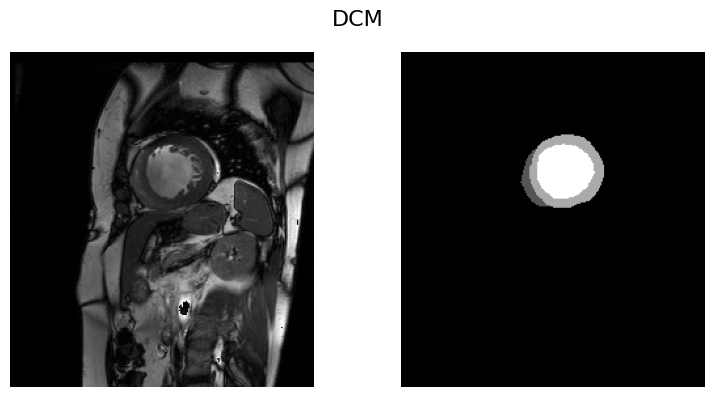
\includegraphics[width=0.8\textwidth]{figures/fig033-01.png}
    \caption*{Fonte: Autor}
    \label{fig:fig033-01}
\end{figure}

\begin{figure}[H]
    \centering
    \caption{Classe HCM + Máscara}
    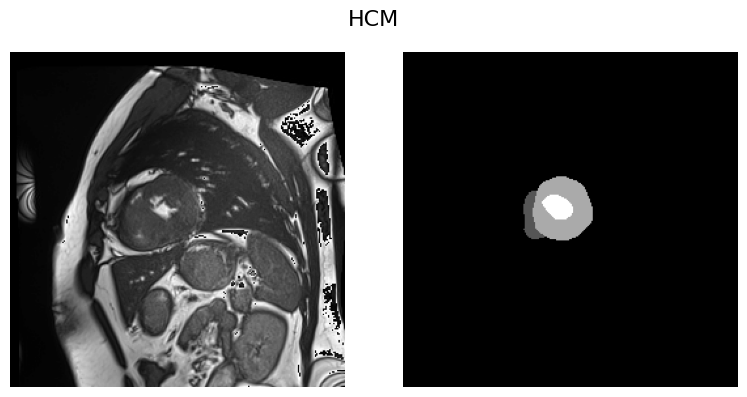
\includegraphics[width=0.8\textwidth]{figures/fig033-02.png}
    \caption*{Fonte: Autor}
    \label{fig:fig033-02}
\end{figure}

\begin{figure}[H]
    \centering
    \caption{Classe NOR + Máscara}
    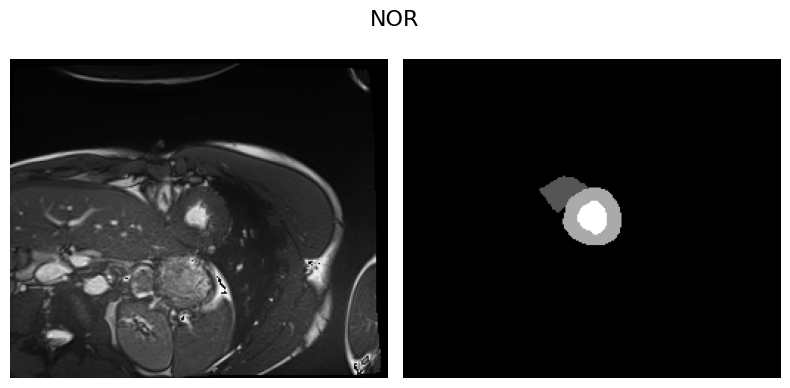
\includegraphics[width=0.8\textwidth]{figures/fig033-03.png}
    \caption*{Fonte: Autor}
    \label{fig:fig033-03}
\end{figure}

% --------------------------------------------------------
\subsection{Conjunto de Dados Sunny} 
\label{subsec:cap4_sunny}

O conjunto de dados Sunny, também conhecidos como \textit{2009 Cardiac MR Left Ventricle Segmentation Challenge data}, consiste em 45 imagens de RM de um grupo misto de pacientes e patologias: saudáveis, hipertrofia, insuficiência cardíaca com infarto e insuficiência cardíaca sem infarto. Um subconjunto desses dados foi utilizado pela primeira vez no desafio de segmentação automatizada do miocárdio a partir de imagens de RM em eixo curto, realizado em um workshop do MICCAI em 2009 \cite{radauEvaluationFrameworkAlgorithms2009}. 

Há quatro grupos patológicos neste conjunto de dados, que foram classificados no seguinte formato:

\begin{enumerate}
    \item Insuficiência cardíaca com infarto (\textbf{IC-I}): grupo com \gls{FE} < $40$\% e evidência de realce tardio com gadolínio (Gd).
    \item Insuficiência cardíaca sem infarto (\textbf{IC}): grupo com \gls{FE} < $40$\% e sem realce tardio com gadolínio.
    \item Hipertrofia do ventrículo esquerdo (\textbf{HIP}): grupo com \gls{FE} normal (> $55$\%) e uma razão de massa do ventrículo esquerdo sobre a área da superfície corporal > $83$ g/m².
    \item Normais (\textbf{NOR}): grupo com \gls{FE} > $55$\% e sem hipertrofia.
\end{enumerate}

\noindent Para o presente trabalho foi utilizado as classes \textbf{HIP} e \textbf{NOR} para classificação de cenário com cardiomiopatia e normal respectivamente. A Tabela \ref{tab:sunny_stats} demonstra como se encontram distribuídos os $45$ pacientes e os valores relacionados as atividades cardiovasculares utilizados para fins de classificação dos pacientes:
\newline

\begin{table}[h!]
\centering
\caption{Estatísticas dos volumes e função do ventrículo esquerdo (média).}
\begin{tabular}{@{}lcccc@{}}
\toprule
\textbf{}  & \textbf{NOR (n=9)} & \textbf{HIP (n=12)} & \textbf{IC (n=12)} & \textbf{IC-I (n=12)} \\ \midrule
\textbf{Vol. Diastólico Final (ml)} & 115.69 (36.89)   & 114.39 (50.46)      & 233.67 (63.21)     & 244.92 (86.02)       \\
\textbf{Vol. Sistólico Final (ml)}  & 43.10 (14.74)    & 43.11 (24.50)       & 158.28 (56.34)     & 174.34 (90.64)       \\
\textbf{Fração de Ejeção (\%)}        & 62.93 (3.65)     & 62.72 (9.22)        & 33.09 (13.07)      & 32.01 (12.27)        \\
\textbf{Massa Ventrículo Esq. (g)} & 130.27 (32.69)   & 175.87 (85.70)      & 193.69 (39.01)     & 201.32 (45.24)       \\ \bottomrule
\end{tabular}
\caption*{Fonte: Adaptado de \cite{radauEvaluationFrameworkAlgorithms2009}.}
\label{tab:sunny_stats}
\end{table}


%--------------------------------------------------------
% \subsection{Conjunto de Dados InCor} 
% \label{subsec:cap4_incor}

% O conjunto de dados \gls{InCor} é composto por casos reais de pacientes que realizaram exames de \gls{RMC} e que foram classificados por especialistas do \gls{InCor} como casos que continham cardiomiopatia hipertrófica, cardiomiopatia dilatada ou nenhuma das duas anomalias. No total foram adquiridos $400$ casos, distribuídos conforme a Figura \ref{fig:fig012}, na qual é possível verificar que a maioria dos casos (69\%) pertencem a indivíduos do sexo masculino, enquanto 31\% pertencem a mulheres. Dentro do grupo de homens verificou-se uma predominância de casos sem anomalia para pacientes com idades entre 21 a 41 anos (25\%), enquanto no grupo de mulheres notou-se que o número maior de casos (21\%) era composto por casos hipertróficos em pacientes com idade entre 42 a 62 anos \cite{bergamascoRECUPERACAOOBJETOSMEDICOS2018}.

% \begin{figure}[htbp]
%     \centering
%     \caption{Distribuição das anomalias entre diferentes gêneros e idades}
%     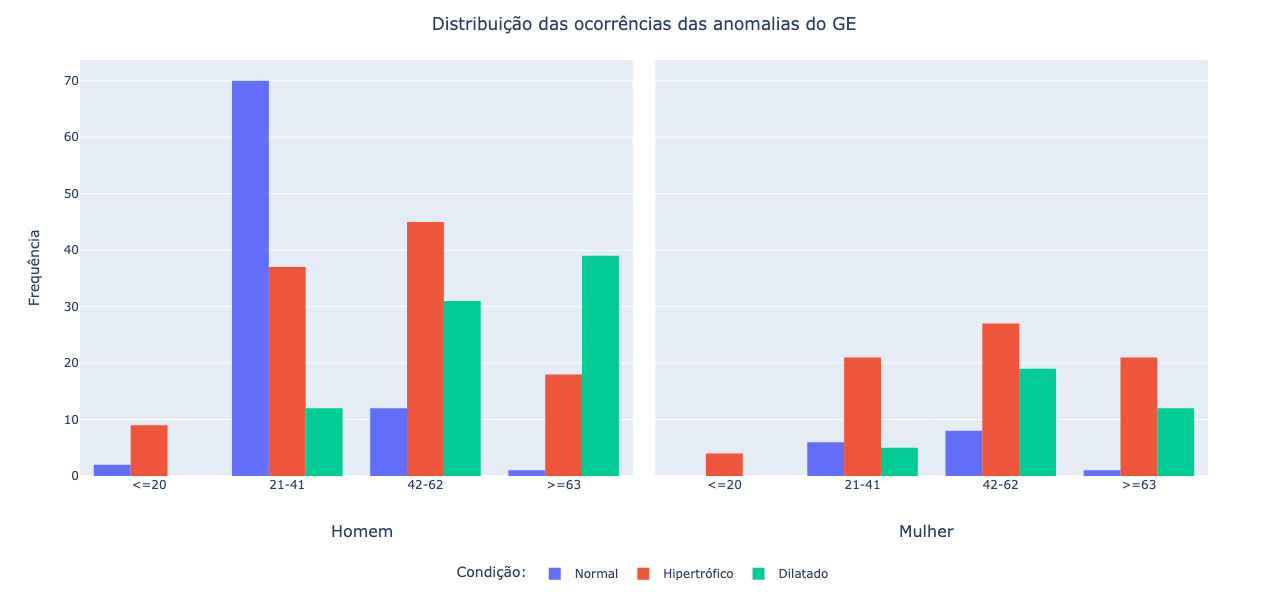
\includegraphics[width=1\textwidth]{figures/fig012.png}
%     \caption*{Fonte: Autor}
%     \label{fig:fig012}
% \end{figure}

%---------------------------------------------------------
\section{PRÉ-PROCESSAMENTO}
\label{subsec:cap4_preprocess}

Na fase de pré-processamento, foi utilizado o conjunto de dados \gls{ACDC}. O \gls{ACDC} originalmente tem cinco classes distintas e foi agrupado de forma que DCM e HCM indicam a classe \gls{CAR} e os demais rótulos NOR, MINF e RV, são classificados como normal. O conjunto de \textit{frames} utilizados são definidos na fase diastólica e a quantidade de \textit{frames} é variada para cada paciente de acordo como consta no conjunto de dados. As características radiômicas são extraídas utilizando a biblioteca \textit{PyRadiomics}\footnote{https://pyradiomics.readthedocs.io}. Utilizando esta ferramenta, pode-se enviar como entrada o volume 3D das imagens cardíacas e suas respectivas máscaras e obter as características manuais extraídas abrangendo textura, forma, escala de cinza, etc. O resultado é um vetor com $\RadiomicFeatures$ características radiômicas. As características profundas são extraídas através de uma rede ResNet50 sem a última camada responsável pela classificação. Este processo é aplicado para cada fatia do volume 3D tanto para imagem cardíaca quanto para sua respectiva máscara tendo como resultado final vetores de tamanho $\DeepFeatures$. 

Seguindo a receita do modelo base, é aplicado o \textit{F-Test} para redução de dimensionalidade das características profundas de $\DeepFeatures$ para $\DeepFeaturesPostLinear$ e das características radiômicas de $\RadiomicFeatures$ para $\text{EMBED}_{size} \in \{24, 48, 64\}$. O valor de $\text{EMBED}_{size}$ varia nas versões adaptadas, sendo considerado um hiperparâmetro, e garante que todos os \textit{embeddings} possuam o mesmo valor. A concatenação é feita na última dimensão para o teste com modelo original e suas variações, e na primeira dimensão para as versões adaptadas. Vale ressaltar que diferente da versão do modelo base que só possui um vetor de características profundas, nas versões adaptadas pode-se ter um vetor adicional referente a máscara com a região de interesse. 

%---------------------------------------------------------
\section{EXTRAÇÃO DE CARACTERÍSTICAS RADIÔMICAS}
\label{subsec:cap4_caracteristicas_radiomicas}

Foram extraídas características radiômicas da fase da diástole\footnote{A diástole corresponde à parte do ciclo cardíaco caracterizada pelo relaxamento muscular e enchimento dos ventrículos \cite{brielerCardiomyopathyOverview2017}}, representada por um conjunto de fatias variando entre $6$ e $18$ \textit{frames}, de cada paciente usando \gls{GLCM} e estatísticas baseadas em histograma. Será aplicado o filtro \gls{LoG} com cinco valores diferentes em cada parte para suavizar as imagens e realçar as bordas. Foi calculado características \gls{GLCM} como contraste, entropia, correlação, homogeneidade e energia para cada filtro \gls{LoG}. Também é calculado características de intensidade como média, variância, média dos percentis (10 e 90), desvio robusto da média absoluta, curtose e assimetria usando estatísticas de primeira ordem. Foram obtidos $\RadiomicFeatures$ características radiômicas para cada paciente dentro da quantidade de fatias extraídas na fase diastólica.

%---------------------------------------------------------
\section{EXTRAÇÃO DE CARACTERÍSTICAS PROFUNDAS}
\label{subsec:cap4_caracteristicas_profundas}
 
Para extrair características profundas das imagens de \gls{RMC}, foi utilizada a arquitetura pré-treinada de um \textit{ResNet50} sem sua última camada totalmente conectada e com os pesos congelados. A \textit{ResNet50} é um modelo de rede neural convolucional profunda com 50 camadas que compreende muitos blocos residuais. Cada bloco contém módulos de convolução e uma conexão de salto que transfere a informação do bloco anterior para o próximo bloco. A conexão de salto ajuda a reter a informação semântica mais básica aprendida nas camadas anteriores, que de outra forma se tornaria abstrata devido à conexão de longa cadeia. A conexão de salto também evita o desaparecimento do gradiente nas camadas mais profundas ao fornecer um caminho alternativo para a retropropagação. A informação da conexão de salto é adicionada à informação calculada em cada bloco \cite{aiSelfAttentionBasedFusion2023}. Ao todo são $\DeepFeatures$ características coletadas da saída deste modelo.

%---------------------------------------------------------
\section{CONCATENAÇÃO}
\label{subsec:cap4_concatenacao}

Em posse das características radiômicas, é aplicado um \textit{F-Test} tanto às $\RadiomicFeatures$ características radiômicas quanto às $\DeepFeatures$ características profundas, reduzindo cada um dos vetores ao espaço dimensional especificado. No método de fusão convencional, simplesmente é concatenado os dois vetores de características como na Equação \ref{eq:concat}, onde \textit{Concat} simplesmente concatena os dois vetores. Unificando os vetores, o resultado é baseado na dimensão escolhida de concatenação escolhida. O resultado é enviado aos mecanismos de atenção, sendo este o bloco de autoatenção no modelo original e o bloco convolucional seguido do bloco de autoatenção no modelo adaptado.

\begin{equation}
F_{hd} = \textit{Concat}(F_h, F_d, dim) \quad dim \in \{0,1\}
\label{eq:concat}
\end{equation}

%---------------------------------------------------------
\section{MÓDULO DE ATENÇÃO SELETIVA}
\label{subsec:cap4_mod_selective_attn}

A atenção seletiva desempenha um papel crucial na melhoria do desempenho de modelos de aprendizado profundo ao permitir que eles foquem em características mais relevantes nas representações internas. Especificamente, o bloco \gls{SE} é projetado para recalibrar adaptativamente os canais das representações, atribuindo pesos maiores às características mais informativas. Esse mecanismo opera em duas etapas principais: primeiro, reduz a dimensionalidade das características globais (\textit{squeeze}) para capturar o contexto geral, e, em seguida, aplica um mecanismo de excitação (\textit{excitation}) para ajustar os pesos de cada canal com base na importância relativa. Ao integrar blocos SE em uma arquitetura, o modelo pode aprimorar sua capacidade de discriminar padrões relevantes e suprimir ruídos ou informações irrelevantes, resultando em maior precisão e eficiência no processamento dos dados \cite{huSqueezeandExcitationNetworks2018}.

Sendo o bloco \gls{SE} adicionado apenas na versão adaptada, visando aprimorar os resultados, o vetor resultante da concatenação é $3\times64$ se assumirmos $\text{EMBED}_{size}$ igual a $64$ e a adição da máscara. Uma camada convolucional 1D é aplicada, com número de canais igual a $16$, \textit{kernel} igual a 3, \textit{stride} igual a $1$ e \textit{padding} igual a $1$ para não diminuir as dimensões após o processamento. Tendo como resultado da primeira convolução $16$ canais, é aplicado o bloco \gls{SE} para identificar os canais mais relevantes e escalar a entrada original. O bloco \gls{SE} possui o parâmetro $r$ de redução de dimensionalidade a ser configurado e foi utilizado o valor $16$ conforme os autores do artigo original sugerem. Outra convolução 1D é aplicada com um único canal, assim tem-se vetor resultante de uma única dimensão que pode servir como entrada para o próximo bloco, o de autoatenção.

%---------------------------------------------------------
\section{MÓDULO DE AUTOATENÇÃO}
\label{subsec:cap4_mod_self_attnn}

O mecanismo de autoatenção foi empregado com a responsabilidade de aprender a importância de cada característica e capturar suas dependências de longo alcance. Como ilustrado na Figura \ref{fig:fig011}, o módulo de autoatenção é utilizado para mapear uma consulta ($Q$), chave ($K$) e valor ($V$) para um valor de atenção. São utilizadas $24$ características concatenadas $F_{hd}$ no modelo original e $\text{EMBED}_{size}$ características nas versões adaptadas. Do vetor resultante, é projetada cada característica em três matrizes aprendíveis: matriz chave $K$, matriz consulta $Q$ e matriz de valor $V$ pelo produto escalar com suas respectivas matrizes de peso $W_{Q}$, $W_{K}$ e $W_{V}$. Logo os valores $Q$, $K$, $V$ são denotados como $W_{Q}F_{gd}$, $W_{K}F_{gd}$, $W_{V}F_{gd}$ respectivamente, onde $W_{Q}$, $W_{K}$ e $W_{V}$ representam a transformação linear para as matrizes $Q$, $K$ e $V$. 

O módulo de autoatenção é definido na Equação \ref{eq:attention}, em que $d_{k}$ é a dimensão do valor de $K$. Sem utilizar operações recorrentes ou convolucionais em específico, o módulo de autoatenção pode modelar as dependências de longo prazo entre as características de entrada.
Este módulo calcula de forma adaptativa os pesos entre as características com base em sua importância e relevância, capturando de forma mais abrangente as associações entre características radiômicas e profundas. Tal processo realça a capacidade expressiva das características fundidas e permite que o modelo foque mais precisamente nas características mais informativas que auxiliam a diagnosticar imagens médicas e reduzir a influência de características irrelevantes nesta previsão. Além disso, o modelo pode alocar dinamicamente atenção a diferentes amostras de imagens de \gls{RMC}. Essa flexibilidade permite com que o modelo se adapte melhor à representação de características de diferentes amostras, melhorando a precisão e a generalização.

A função de perda utilizada utilizada no modelo é a função de entropia cruzada binária, do termo  \gls{BCE}, que é calculada pela Equação. \ref{eq:bce} onde $\mathcal{L}_{bce}$ denota o \gls{BCE}, $N$ denota o número de imagens de \gls{RMC}, $r$ denota a classe alvo de \gls{CAR} e $\hat{r}$ o valor previsto pelo modelo de \gls{CAR}, 1 indica indícios de \gls{CAR} e 0 sua ausência.

\begin{equation}
\mathcal{L}_{bce} = -\frac{1}{N} \sum_{i=1}^N
(r_i \ln \hat{r}_i + (1 - r_i) \ln (1 - \hat{r}_i))
\label{eq:bce}
\end{equation}

%---------------------------------------------------------
\section{MÉTRICAS}
\label{subsec:cap4_metrics}
Para medir o desempenho da solução serão aplicadas as seguintes métricas: acurácia, precisão, revocação expressas pelas Equações \ref{eq:acc}, \ref{eq:precision} e \ref{eq:recall} respectivamente.

Também foi calculada a \gls{AUC}, que consistem em um gráfico com a habilidade de validar um classificador binário. Esta curva é criada plotando, em gráfico, a taxa de verdadeiros positivos (TPR) contra a taxa de falsos positivos (FPR) em diversos limites contínuos de decisão. A equação da \gls{AUC} é apresentada na Equação \ref{eq:auc} em formato contínuo embora seja prática comum discretizá-lo.


\begin{equation}
  \textit{Acurácia} = \frac{\textit{TP} + \textit{TN}}{\textit{TP} + \textit{TN} + \textit{FP} + \textit{FN}}
  \label{eq:acc}
\end{equation}

\begin{equation}
  \textit{Precisão} = \frac{\textit{TP}}{\textit{TP} + \textit{FP}}
  \label{eq:precision}
\end{equation}

\begin{equation}
  \textit{Revocação} = \frac{\textit{TP}}{\textit{TP} + \textit{FN}}
  \label{eq:recall}
\end{equation}

\begin{equation}
  \text{AUC} = \int_{x=0}^{1} \text{TPR}(\text{FPR}^{-1}(x)) \ \, d(x)
  \label{eq:auc}
\end{equation}

%---------------------------------------------------------
\section{ARQUITETURA PROPOSTA}
\label{subsec:cap4_architecture}

% A arquitetura proposta é composta por: extração de características radiômicas e profundas; redução de dimensionalidade para que ambas possuam tamanhos similares, aplicação dos mecanismos de atenção seletivo e autoatenção e classificação binária do resultado.

O esquemático da arquitetura proposta é observado na Figura \ref{fig:fig011}. As características profundas são extraídas das imagens e máscaras via ResNet50 e sofrem uma transformação linear com o valor de $\DeepFeaturesPostLinear$ conforme trabalho original. As características radiômicas são extraídas via aplicação de diversos modelos estatísticos resultando no valor de $\RadiomicFeatures$. Um conjunto de F-Test são aplicados nos vetores para garantir que possuam o mesmo tamanho, tamanho este decidido pelo parâmetro $\text{EMBED}_{size}$. As características selecionadas são concatenadas e enviadas ao módulo de convolução composto respectivamente por: convolução 1D, bloco \gls{SE} e convolução 1D. A primeira convolução converte o número de canais para $16$, o bloco \gls{SE} mantém a dimensionalidade e a segunda convolução converte os canais de $16$ para $1$. O processo segue no módulo se autoatenção e, por fim, uma camada linear com um único neurônio faz a classificação binária. A arquitetura proposta neste trabalho tem como base o trabalho de \cite{aiSelfAttentionBasedFusion2023}.
\newline

\begin{figure}[H]
    \centering
    \caption{Arquitetura Proposta}
    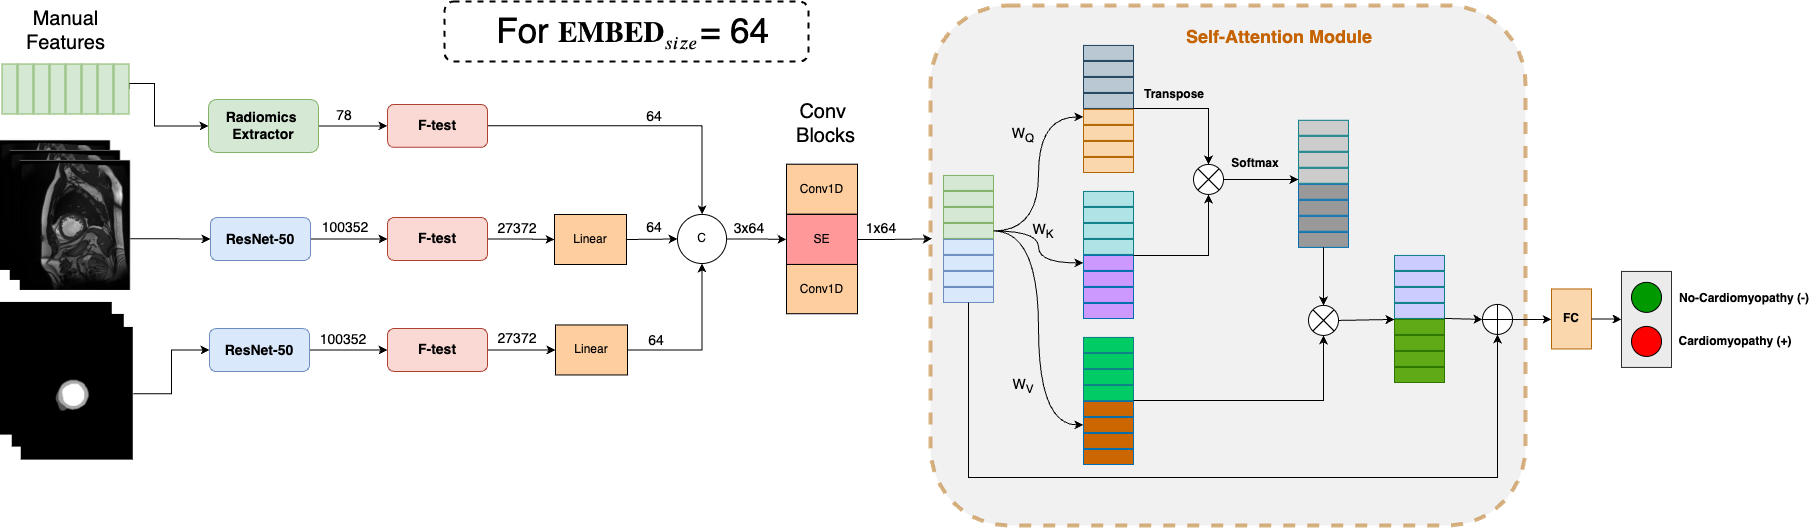
\includegraphics[width=1.02\textwidth]{figures/fig011.png}
    \caption*{Fonte: Autor}
    \label{fig:fig011}
\end{figure}

%---------------------------------------------------------
\section{CONSIDERAÇÕES FINAIS DO CAPÍTULO}
\label{sec:cap4_consideracoes_finais}

Como considerações, destacam-se o uso de base de dados pública, com dados de pacientes incluindo o conjuntos de fatias que identificam a ação de sístole e diástole do coração. É aplicado pré-processamento do qual são extraídas as características radiômicas, características estas que analisam textura, níveis e variações dos tons de cinza incluindo diversas estatísticas como de primeira ordem e o \gls{GLCM}. Ainda em fase de pré-processamento é extraída as características profundas oriundas do modelo de visão \textit{ResNet50}, com os pesos treinados na base de dados da \textit{ImageNet}. 

A adaptação inicia ao se adicionar os \textit{embeddings} das máscaras também ao modelo, poder variar o vetor tamanho dos vetores de características, pois no modelo original eram apenas $12$. Os vetores são então extraídos via \textit{F-Test}, concatenados e inseridos no novo bloco convolucional. Este bloco possui um bloco \gls{SE} responsável pela atenção seletiva, dando importância aos canais mais pertinentes. Por fim o módulo de autoatenção, confere as relações intrínsecas das transformações anteriores, identificando as características mais determinantes independente de espacialidade e a classificação é apresentada.
